
%***************************************************************************
%
% CreditCruncher - A portfolio credit risk valorator
% Copyright (C) 2004 Gerard Torrent
%
% This program is free software; you can redistribute it and/or
% modify it under the terms of the GNU General Public License
% as published by the Free Software Foundation; either version 2
% of the License.
%
% This program is distributed in the hope that it will be useful,
% but WITHOUT ANY WARRANTY; without even the implied warranty of
% MERCHANTABILITY or FITNESS FOR A PARTICULAR PURPOSE.  See the
% GNU General Public License for more details.
%
% You should have received a copy of the GNU General Public License
% along with this program; if not, write to the Free Software
% Foundation, Inc., 59 Temple Place - Suite 330, Boston, MA 02111-1307, USA.
%
%
% resolution.tex - TeX documentation file
% --------------------------------------------------------------------------
%
% 2005/01/22 - Gerard Torrent [gerard@fobos.generacio.com]
%   . initial release
%
%***************************************************************************

\chapter{Resoluci\'on del problema}
\label{sec:resolution}

TODO: que es lo que esperamos: flexibilidad, resultados finos, paralelismo 
con la valoracion del riesgo de mercado (pe. valoracion de opciones)

%---------------------------------------------------------------------------

\section{Hip\'otesis}

A continuaci\'on se enumeran las hip\'otesis duras. 
\begin{enumerate}
\item Los fallidos no se recuperan.
\item La \'unica fuente de riesgo considerada es el riesgo de impago. No se 
contemplan otros tipos de riesgos como la variaci\'on de tipos de inter\'es, 
de mercado, operacional, reputacional, etc.
\item La descripci\'on de cada activo (cashflow, exposici\'on y recuperaci\'on) 
se conoce de antemano y no var\'ia a lo largo de la simulaci\'on. En particular,
el valor del activo solo depende de si el cliente hace fallido, no del rating
que pueda tener el cliente. Por otra parte, la recuperaci\'on no puede variar en 
funci\'on de la evoluci\'on del rating de otro cliente.
\item El rating de un cliente no depende del rating de otro cliente de otra 
forma forma que no sea la correlaci\'on entre sectores. Esta restricci\'on no 
permite tratar el rating de las empresas subsidiarias en funci\'on del rating 
de la empresa matriz.
\end{enumerate}

A continuaci\'on se enumeran las hip\'otesis blandas. 
\begin{enumerate}
\item Los intervalos de tiempo considerado se encuentran equiespaciados. Esto 
permite simplificar los datos de entrada y el n\'umero de matrices de 
transici\'on a considerar.
\item La matriz de transici\'on no var\'ia a lo largo del tiempo. Se aplica 
la misma matriz de transici\'on anual para pasar de $t_0$ a $t_1$ que para 
pasar de $t_{19}$ a $t_{20}$. Esto permite simplificar los datos de entrada y 
el n\'umero de matrices de transici\'on a considerar.
\end{enumerate}

%---------------------------------------------------------------------------

\section{Reparto del tiempo}


%---------------------------------------------------------------------------

\section{El m\'etodo de Monte Carlo}



%---------------------------------------------------------------------------

\section{C\'opulas. Variables aleatorias correlacionadas}

\subsection{Errores comunes sobre la correlaci\'on}

\paragraph{Definici\'on.}
Una copula es la funci\'on de distribuci\'on de un vector aleatorio sobre 
$\Re^n$ donde las funciones de distribuci\'on marginales son $U[0,1]$. 
\begin{displaymath}
C(u_1, \cdots, u_n) = P\{U_1 \leq u_1, \cdots, U_n \leq u_n\}
\end{displaymath}

\paragraph{Proposici\'on.}
$C$ es una c\'opula $\iff C:[0,1]^n \to [0,1]$ y cumple las siguientes 
propiedades:
\begin{itemize}
\item $C(x_1, \cdots, x_n)$ es creciente en cada componente $x_i$
\item $C(1, \cdots, 1, x_i, 1, \cdots, 1) = x_i \quad \forall i \in \{1, \cdots, n\}, x_i \in [0,1]$
\item $\forall (a_1, \cdots, a_n) \in [0,1]^n$ y $\forall (b_1, \cdots, b_n) \in [0,1]^n$ con
$a_i \leq b_i$ se cumple:
\begin{displaymath}
\sum_{i_1=1}^{2} \cdots \sum_{i_n=1}^{2} (-1)^{i_1+\cdots+x_n} C(x_{1i_1},\cdots,x_{ni_n}) \geq 0
\end{displaymath}
\noindent siendo $x_{j1}=a_j$ y $x_{j2}=b_j$ $\quad \forall j \in \{1, \cdots, n\}$
\end{itemize}

\paragraph{Generaci\'on de c\'opulas gausianas.}

\begin{figure}[!hb]
\begin{center}
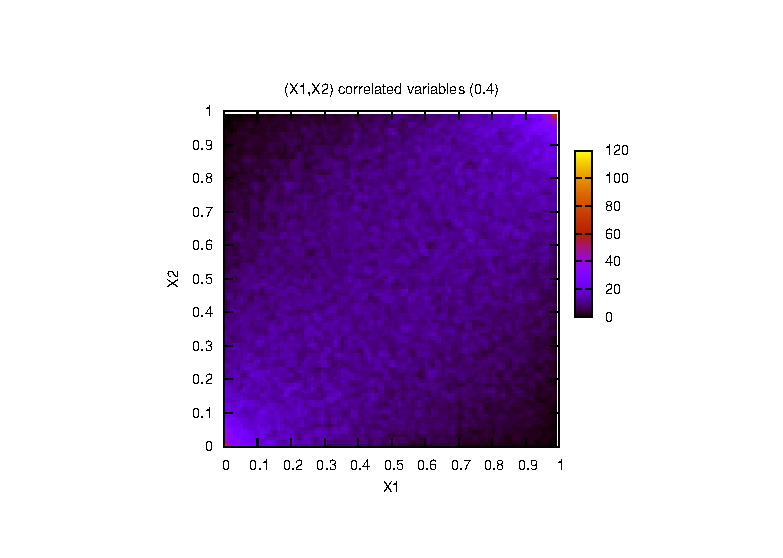
\includegraphics[height=5cm, angle=0]{./images/copula.eps}
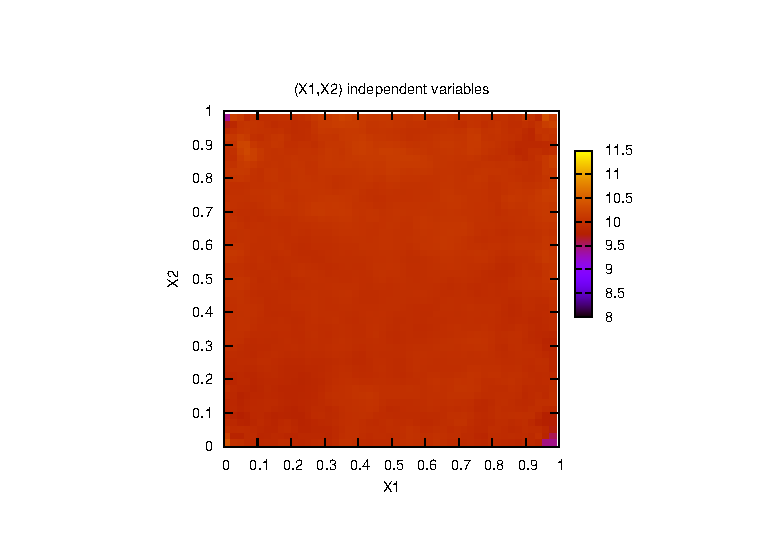
\includegraphics[height=5cm, angle=0]{./images/uniform.eps}
\caption{Bivariate distribution plot with correlation and independent}
\label{copulas}
\end{center}
\end{figure}

%---------------------------------------------------------------------------

\section{Algoritmo de resoluci\'on}

